\documentclass[tikz,border=4pt,11pt]{standalone}
\usepackage{amsmath}
\definecolor{ink}{RGB}{42,52,64}
\definecolor{first}{RGB}{146,79,26}
\definecolor{second}{RGB}{26,99,111}

% The graph on [7] with edges 12,23,13,34,45,35,56,67, drawn six times.
% Each copy highlights one matching with three edges; the six covered
% vertex sets are the bases 123456, 123467, 123567, 124567, 134567, 234567
% of the matching matroid.  The uncovered vertex is drawn grey.
% Each basis is covered by exactly one matching.

\begin{document}
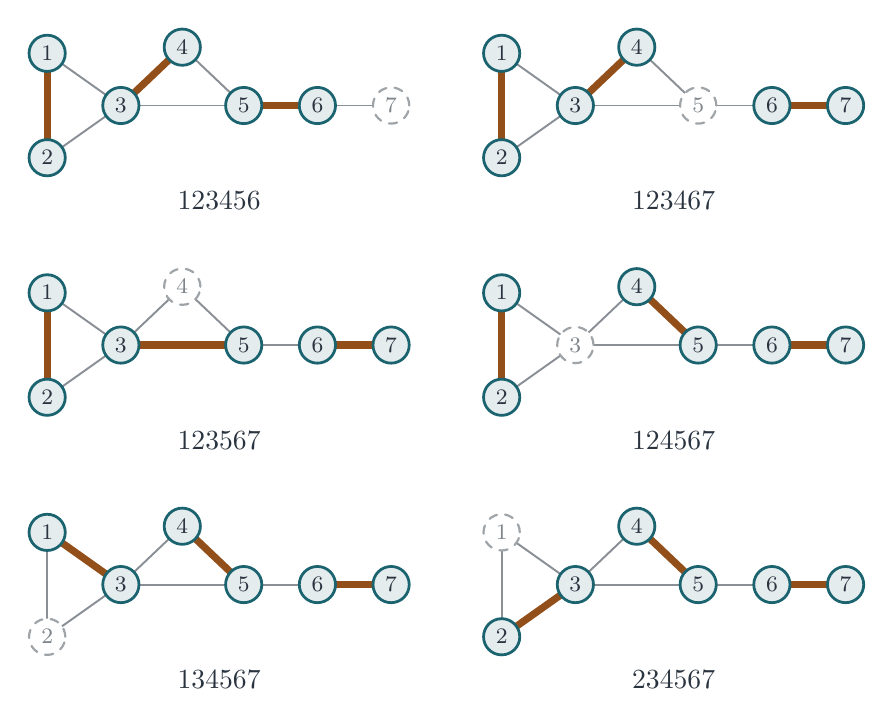
\begin{tikzpicture}[text=ink,line cap=round,x=.78cm,y=.78cm,
  vtx/.style={circle,draw=second,fill=second!12,line width=1pt,inner sep=0pt,
    minimum size=4.6mm,font=\footnotesize},
  uncov/.style={circle,draw=ink!45,fill=white,dashed,line width=.8pt,inner sep=0pt,
    minimum size=4.6mm,font=\footnotesize,text=ink!60}]
% #1: uncovered vertex, #2: matching edges a/b, #3: basis
\newcommand{\panel}[3]{%
  \coordinate (v1) at (0,.85);
  \coordinate (v2) at (0,-.85);
  \coordinate (v3) at (1.2,0);
  \coordinate (v4) at (2.2,.95);
  \coordinate (v5) at (3.2,0);
  \coordinate (v6) at (4.4,0);
  \coordinate (v7) at (5.6,0);
  \foreach \a/\b in {1/2,2/3,1/3,3/4,4/5,3/5,5/6,6/7}
    \draw[ink!55,line width=.7pt] (v\a) -- (v\b);
  \foreach \a/\b in {#2}
    \draw[first,line width=2.6pt] (v\a) -- (v\b);
  \foreach \v in {1,...,7} {
    \ifnum\v=#1
      \node[uncov] at (v\v) {$\v$};
    \else
      \node[vtx] at (v\v) {$\v$};
    \fi
  }
  \node at (2.8,-1.55) {$#3$};
}

\begin{scope}[shift={(0,0)}]\panel{7}{1/2,3/4,5/6}{123456}\end{scope}
\begin{scope}[shift={(7.4,0)}]\panel{5}{1/2,3/4,6/7}{123467}\end{scope}
\begin{scope}[shift={(0,-3.9)}]\panel{4}{1/2,3/5,6/7}{123567}\end{scope}
\begin{scope}[shift={(7.4,-3.9)}]\panel{3}{1/2,4/5,6/7}{124567}\end{scope}
\begin{scope}[shift={(0,-7.8)}]\panel{2}{1/3,4/5,6/7}{134567}\end{scope}
\begin{scope}[shift={(7.4,-7.8)}]\panel{1}{2/3,4/5,6/7}{234567}\end{scope}
\end{tikzpicture}
\end{document}
